\documentclass[11pt]{article}
\usepackage[margin=0.9in]{geometry}
\usepackage{booktabs}
\usepackage{graphicx}
\usepackage{xcolor}
\usepackage{amsmath}
\usepackage{hyperref}
\usepackage{float}

\definecolor{good}{HTML}{27AE60}
\definecolor{ok}{HTML}{F39C12}
\definecolor{bad}{HTML}{E74C3C}

\title{Dynamic P\textsubscript{env} Calibration Report\\[0.3em]\large Wavefront Calibration Rounds W65--W74}
\author{Anton Star --- SSWD-EvoEpi Project}
\date{March 4, 2026}

\begin{document}
\maketitle

\section{Executive Summary}

\textbf{Dynamic P\textsubscript{env} creates the north-south recovery gradient that static P\textsubscript{env} could not.} W71 (floor=100, $\delta$=0.02) achieves the best RMSE of any run to date (\textbf{0.692}), with SS-S dropping from 22\% (static) to \textbf{1.6\%} (target 5\%) and CA-N from 1.3\% to \textbf{0.3\%} (target 0.1\%). However, AK recovery is now too low (10.5\% vs target 50\%). The mechanism works --- it just needs parameter adjustment to lift the overall recovery level while preserving the gradient.

\begin{figure}[H]
\centering
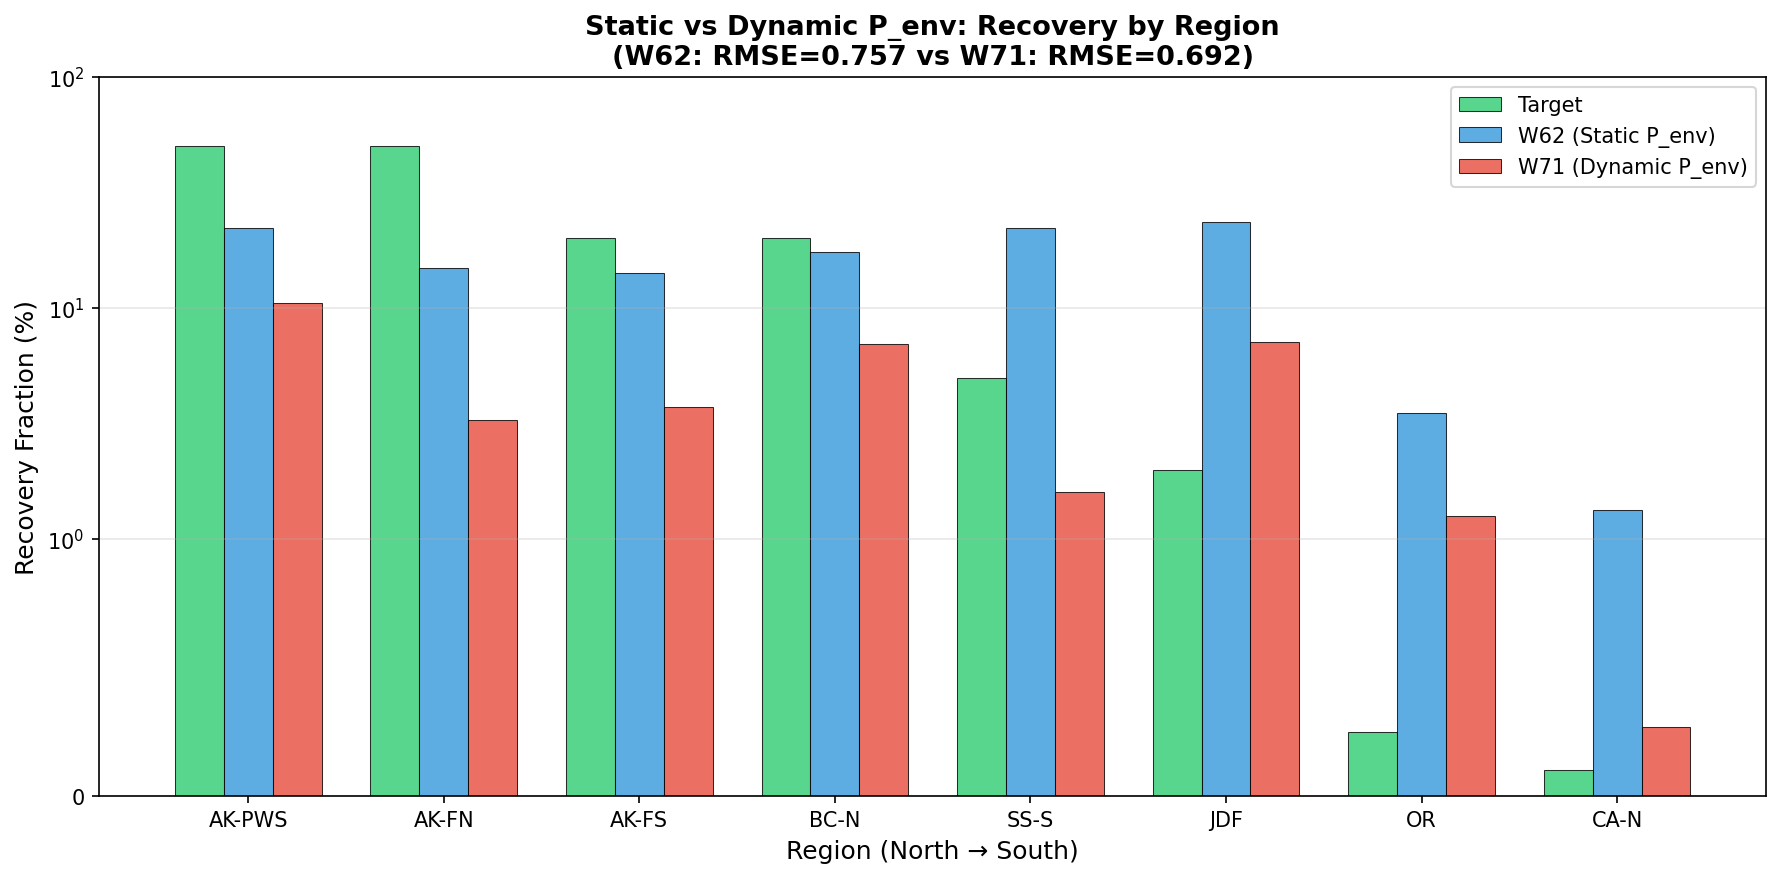
\includegraphics[width=\textwidth]{figures/fig4_static_vs_dynamic.png}
\caption{Recovery fractions by region: targets (green), static P\textsubscript{env} W62 (blue), and dynamic P\textsubscript{env} W71 (red). Dynamic P\textsubscript{env} creates the gradient that static P\textsubscript{env} could not, but overall levels are too suppressed.}
\end{figure}

\section{Mechanism}

Dynamic P\textsubscript{env} replaces the static \texttt{P\_env\_max} with a per-node vibrio reservoir:

\begin{equation}
P_\text{env,pool}(t+1) = \max\left(0,\ P_\text{env,pool}(t) + \alpha_\text{env} \cdot S_\text{shed} - \delta_\text{env} \cdot P_\text{env,pool}(t)\right)
\end{equation}

\begin{equation}
P_\text{env,total} = \underbrace{P_\text{env,floor} \cdot \text{VBNC}(T) \cdot g(T) \cdot s(\text{sal})}_{\text{community floor}} + P_\text{env,pool}
\end{equation}

The community floor is SST-modulated via the VBNC sigmoid: warm southern waters ($\sim$15--18$^\circ$C) maintain $\sim$10$\times$ higher baseline vibrio concentrations than cold northern waters ($\sim$5--8$^\circ$C in winter). This creates \textbf{differential disease persistence}.

\section{Design Matrix}

All runs use W62 base: CDT=1000, K$_{1/2}$=400K, wfDP=300, wfRange=3000, P\textsubscript{env,max}=2000, k\textsubscript{vbnc}=2.0.

\begin{table}[H]
\centering
\begin{tabular}{lcccl}
\toprule
Run & P\textsubscript{env,floor} & $\delta_\text{env}$ & $\alpha_\text{env}$ & Half-life \\
\midrule
W65--W67 & 25 & 0.02 / 0.05 / 0.1 & 0.1 & 35d / 14d / 7d \\
W68--W70 & 50 & 0.02 / 0.05 / 0.1 & 0.1 & 35d / 14d / 7d \\
W71--W73 & 100 & 0.02 / 0.05 / 0.1 & 0.1 & 35d / 14d / 7d \\
W74 & 50 & 0.05 & 0.2 & 14d \\
\bottomrule
\end{tabular}
\end{table}

\section{Results: Recovery Fractions}

\begin{table}[H]
\centering
\small
\begin{tabular}{lc|cccccccc}
\toprule
& & \multicolumn{8}{c}{Recovery Fraction (\%)} \\
Run & RMSE & AK-PWS & AK-FN & AK-FS & BC-N & SS-S & JDF & OR & CA-N \\
\midrule
Target & --- & 50.0 & 50.0 & 20.0 & 20.0 & 5.0 & 2.0 & 0.25 & 0.1 \\
\midrule
W65 & 0.970 & 8.8 & 14.5 & 5.8 & 5.3 & 17.2 & 22.8 & 6.4 & 4.3 \\
W66 & 1.357 & 42.1 & 40.7 & 40.5 & 32.0 & 55.1 & 62.8 & 30.8 & 42.0 \\
W67 & 1.508 & 79.3 & 62.3 & 58.9 & 66.2 & 76.0 & 69.8 & 62.5 & 71.2 \\
\midrule
W68 & 0.942 & 14.5 & 3.3 & 8.5 & 7.2 & 5.6 & 14.3 & 4.9 & 4.3 \\
W69 & 1.269 & 38.2 & 37.0 & 30.4 & 33.4 & 40.0 & 54.5 & 25.0 & 26.9 \\
W70 & 1.460 & 74.9 & 67.1 & 57.8 & 62.2 & 61.7 & 67.1 & 56.5 & 54.8 \\
\midrule
\textbf{W71} & \textbf{0.692} & 10.5 & 3.3 & 3.7 & 7.0 & \textbf{1.6} & 7.1 & 1.3 & \textbf{0.3} \\
W72 & 1.197 & 33.0 & 32.9 & 25.2 & 31.3 & 24.6 & 31.7 & 23.6 & 22.5 \\
W73 & 1.402 & 71.1 & 62.9 & 47.1 & 60.3 & 60.9 & 61.6 & 47.3 & 39.5 \\
\midrule
W74 & 0.881 & 10.9 & 10.4 & 8.3 & 11.7 & 12.8 & 18.8 & 5.5 & 3.0 \\
\bottomrule
\end{tabular}
\caption{W65--W74 recovery fractions. W71 achieves lowest RMSE (0.692) with strong southern suppression. Best prior static run (W62) had RMSE=0.757 with flat gradient.}
\end{table}

\section{Recovery Time Series}

\begin{figure}[H]
\centering
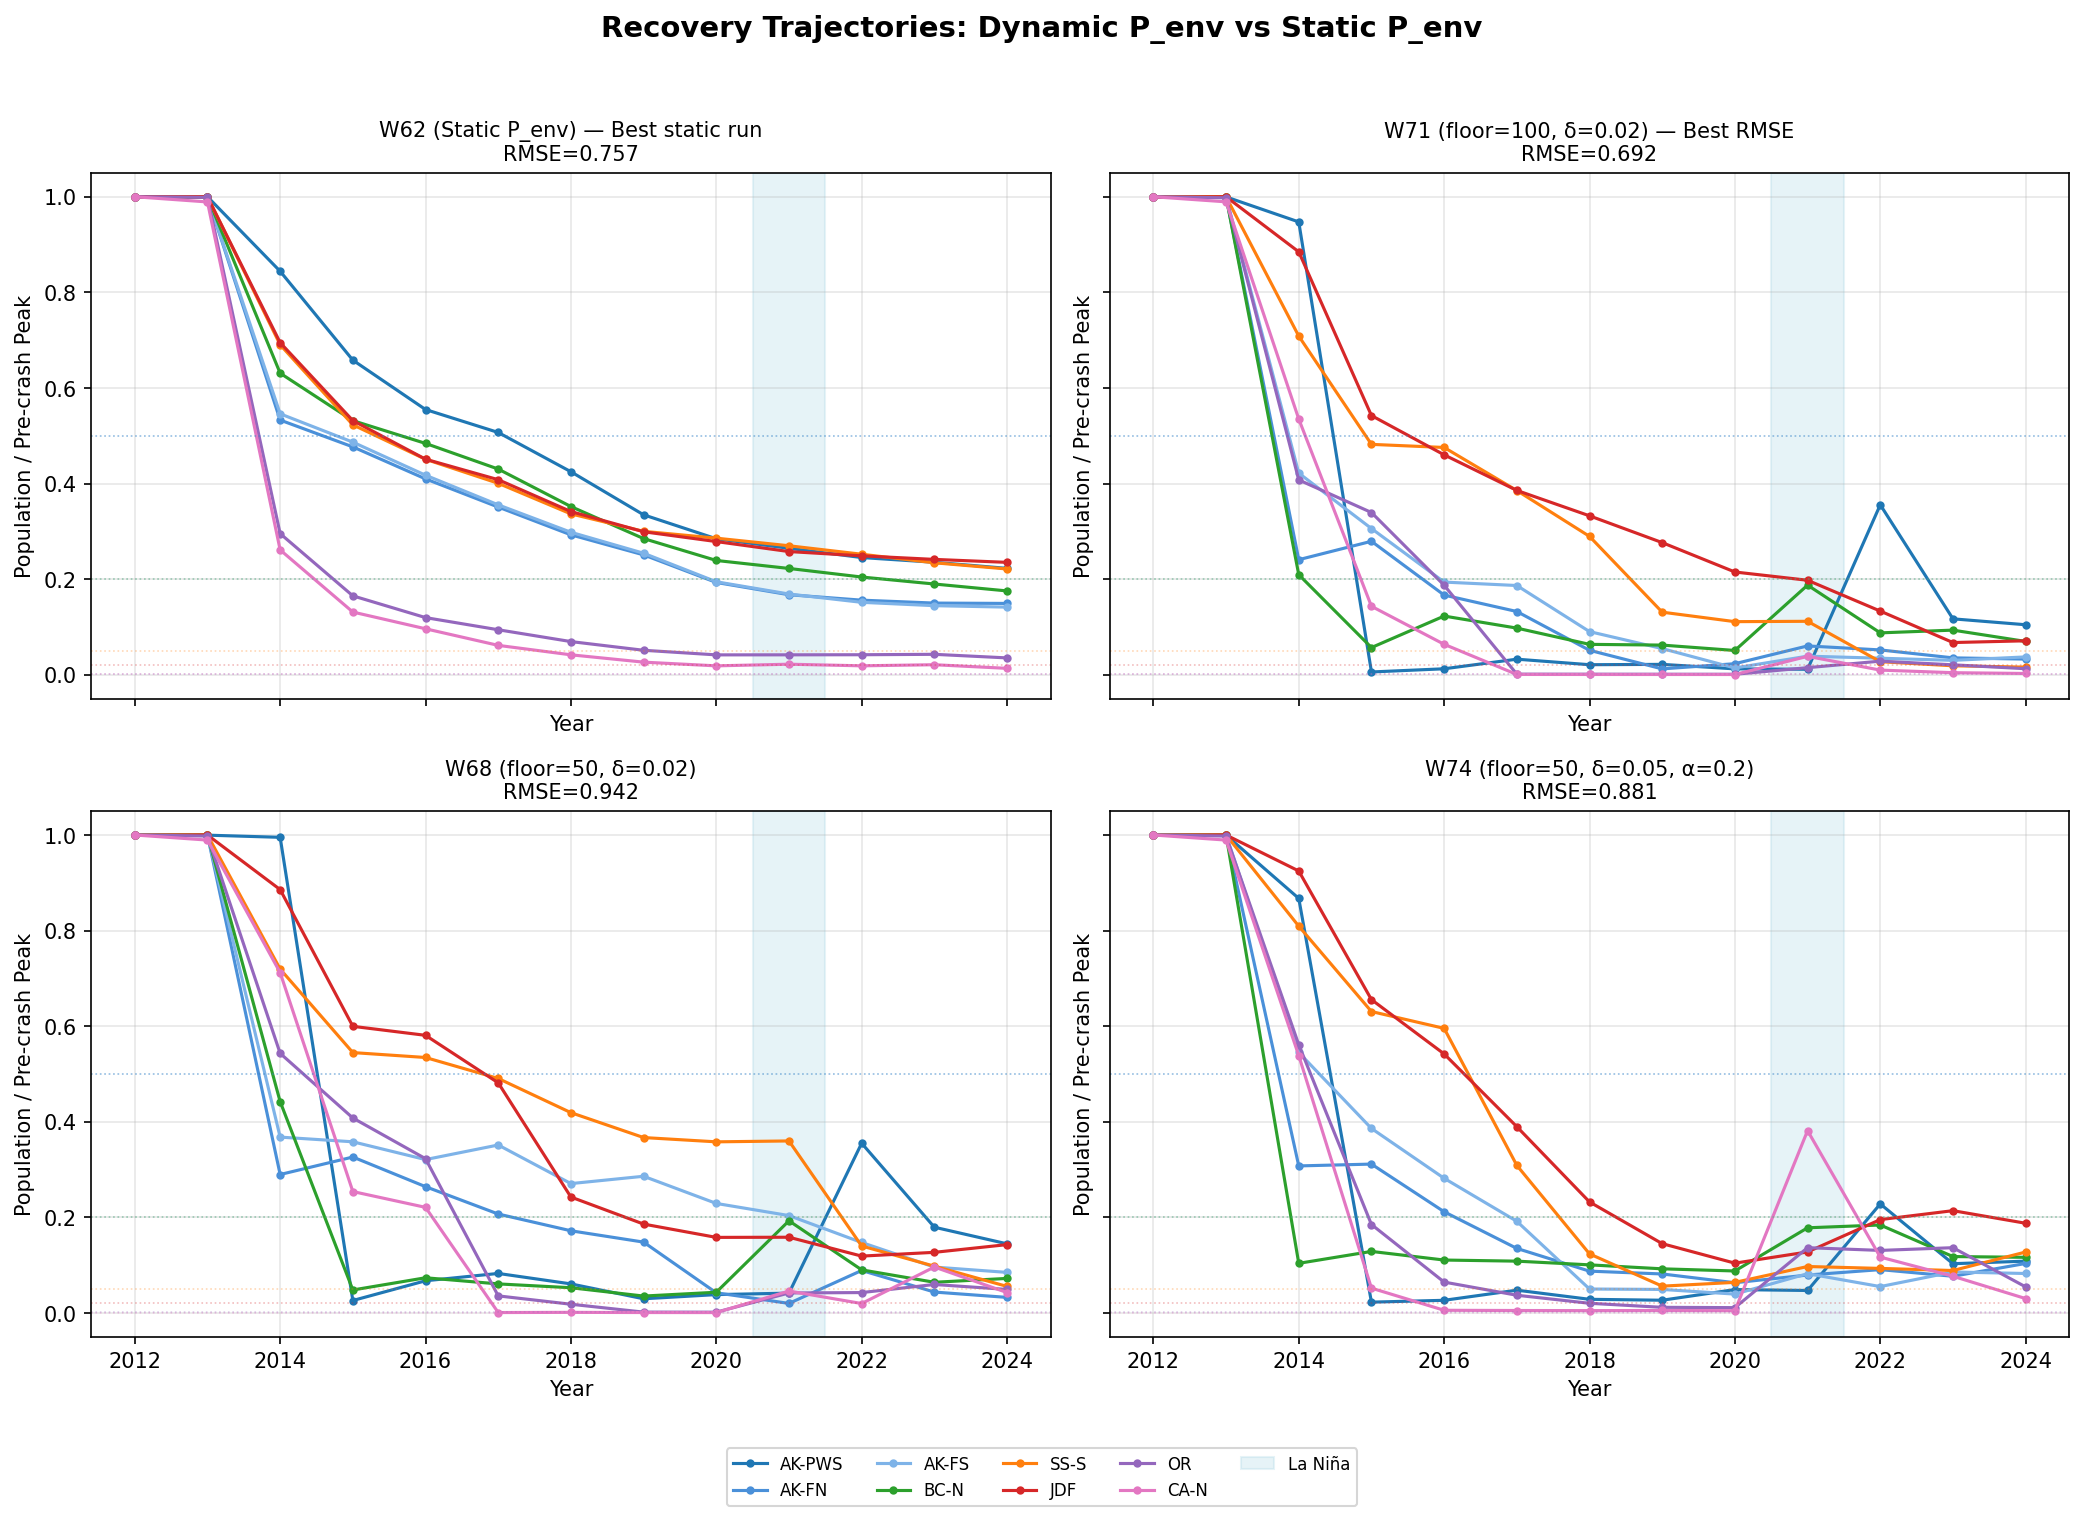
\includegraphics[width=\textwidth]{figures/fig1_recovery_timeseries.png}
\caption{Recovery trajectories for key runs. W62 (static, top-left) shows all regions recovering to $\sim$20\%. W71 (dynamic, top-right) shows clear north-south gradient: AK-PWS rebounds then oscillates while SS-S and CA-N remain near zero. Blue shading indicates the 2020--2021 La Ni\~na cooling event.}
\end{figure}

\begin{figure}[H]
\centering
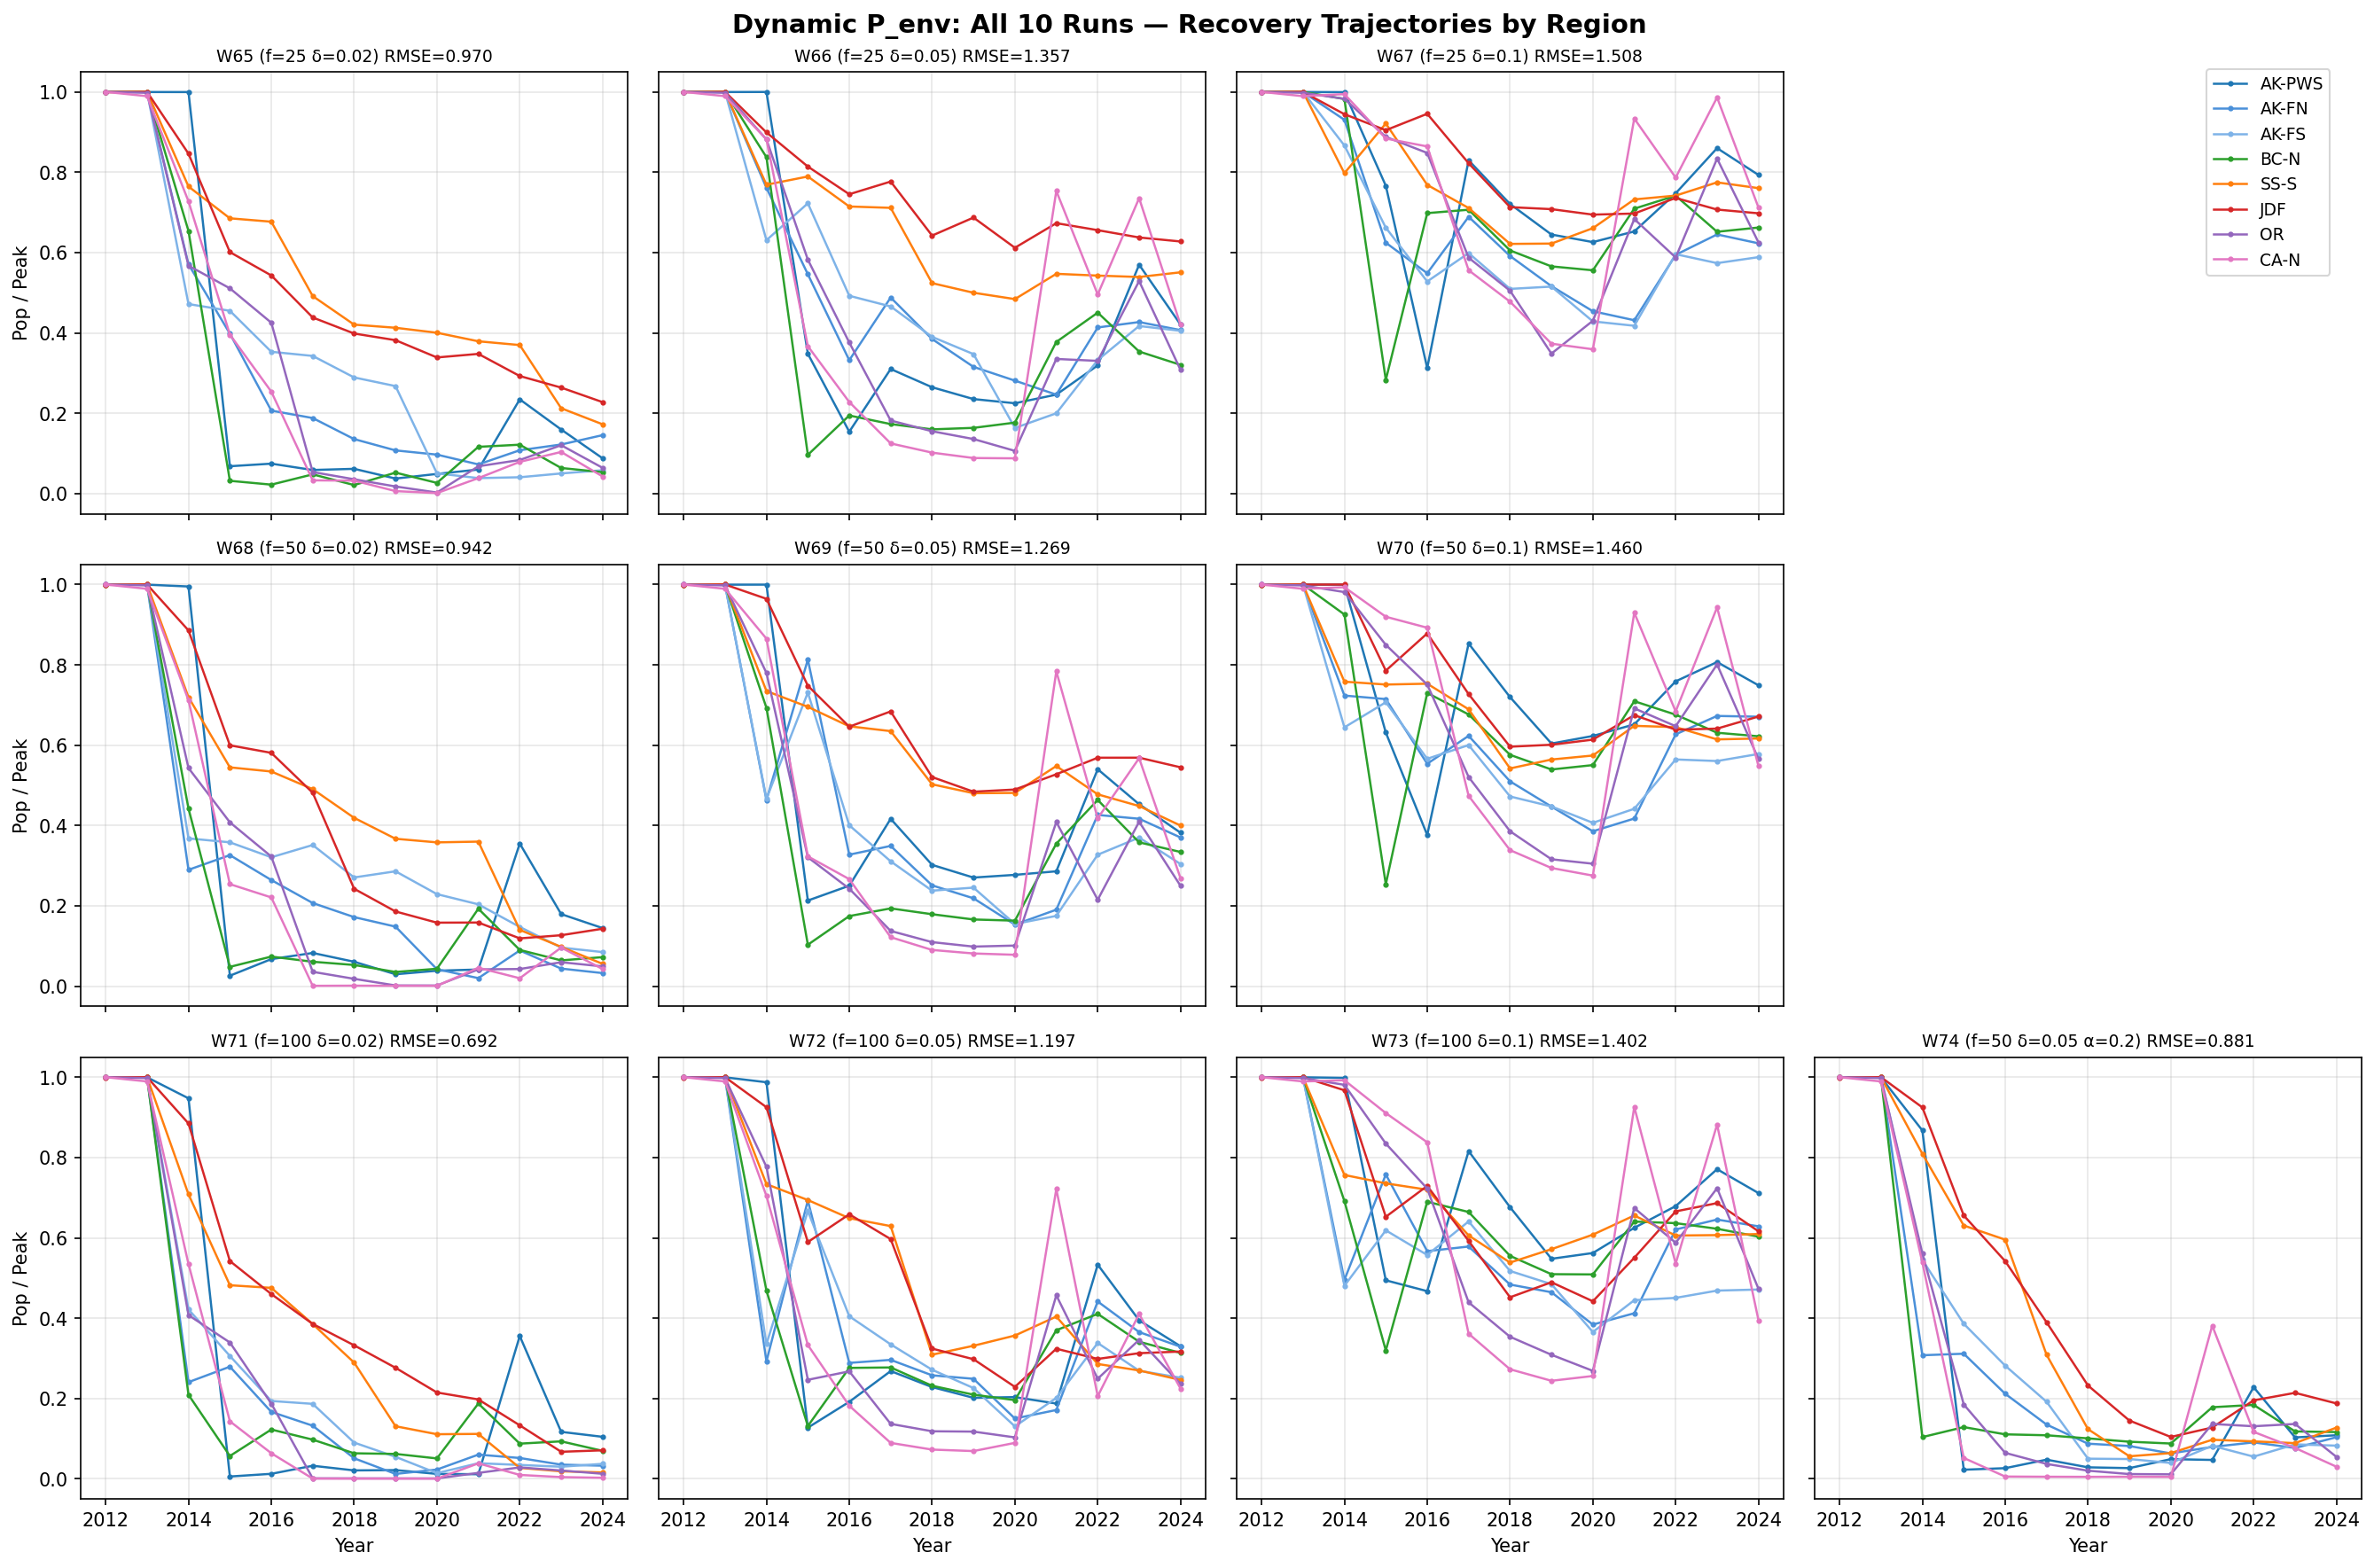
\includegraphics[width=\textwidth]{figures/fig2_all_runs_timeseries.png}
\caption{All 10 dynamic P\textsubscript{env} runs. Left column ($\delta$=0.02): strong differentiation. Middle ($\delta$=0.05): moderate. Right ($\delta$=0.1): nearly flat --- pool decays too fast to maintain suppression.}
\end{figure}

\section{Key Findings}

\subsection{$\delta_\text{env}$ is the dominant parameter}

\begin{figure}[H]
\centering
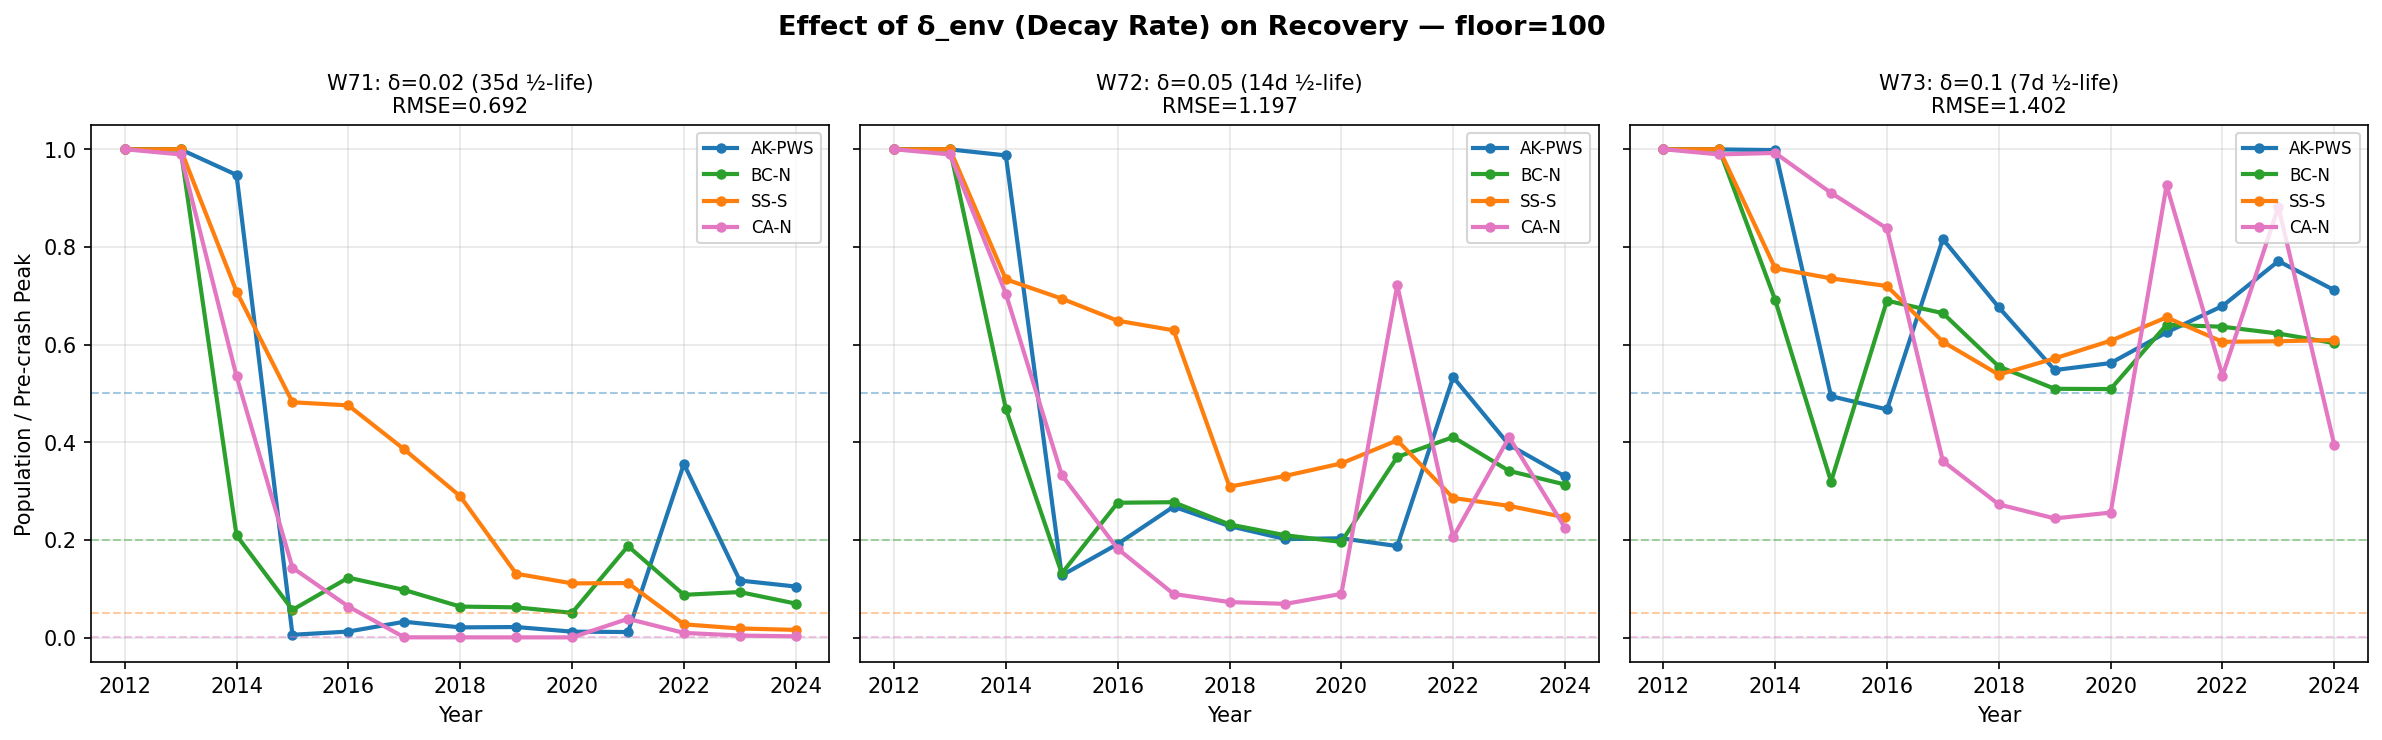
\includegraphics[width=\textwidth]{figures/fig3_delta_effect.png}
\caption{Effect of decay rate at floor=100. Left ($\delta$=0.02): clear gradient, south suppressed. Center ($\delta$=0.05): moderate suppression. Right ($\delta$=0.1): gradient collapses --- pool decays within a week. Dashed lines show calibration targets.}
\end{figure}

\begin{figure}[H]
\centering
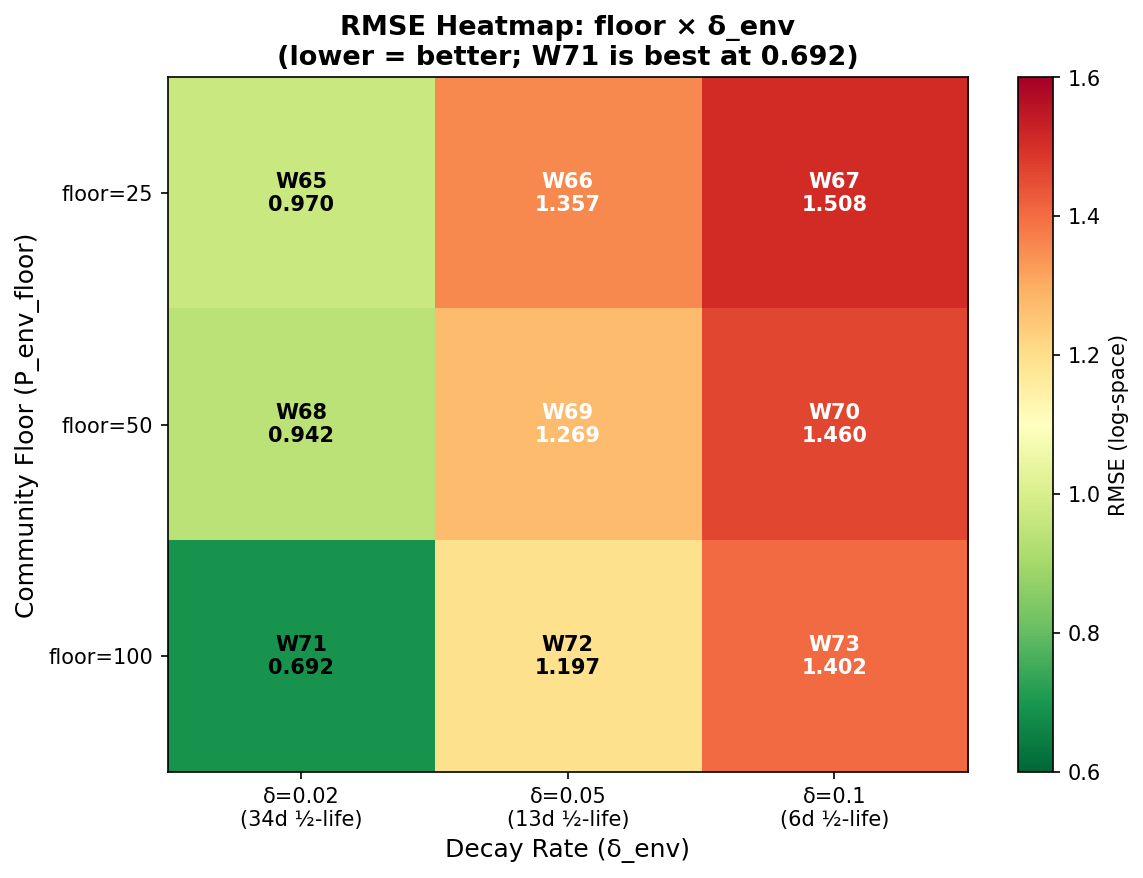
\includegraphics[width=0.65\textwidth]{figures/fig6_rmse_heatmap.png}
\caption{RMSE heatmap across the floor $\times$ $\delta$ parameter space. Optimal region is bottom-left (high floor, slow decay). W71 (floor=100, $\delta$=0.02) achieves RMSE=0.692.}
\end{figure}

\textbf{Biological interpretation}: \textit{V.~pectenicida} in marine biofilms and sediments persists for weeks to months, not days. A 35-day half-life ($\delta$=0.02) is consistent with literature on vibrio environmental persistence in temperate marine systems.

\subsection{Dynamic P\textsubscript{env} creates the gradient}

\begin{table}[H]
\centering
\begin{tabular}{lcccc}
\toprule
Run & Type & AK-PWS & SS-S & North/South Ratio \\
\midrule
W62 (best static) & Static & 22.3\% & 22.1\% & 1.01$\times$ (flat) \\
\textbf{W71 (best dynamic)} & Dynamic & 10.5\% & 1.6\% & \textbf{6.6$\times$} (gradient) \\
\midrule
Target & --- & 50.0\% & 5.0\% & 10$\times$ \\
\bottomrule
\end{tabular}
\caption{Static P\textsubscript{env} produces zero gradient. Dynamic P\textsubscript{env} achieves 6.6$\times$ gradient (target $\sim$10$\times$).}
\end{table}

\begin{figure}[H]
\centering
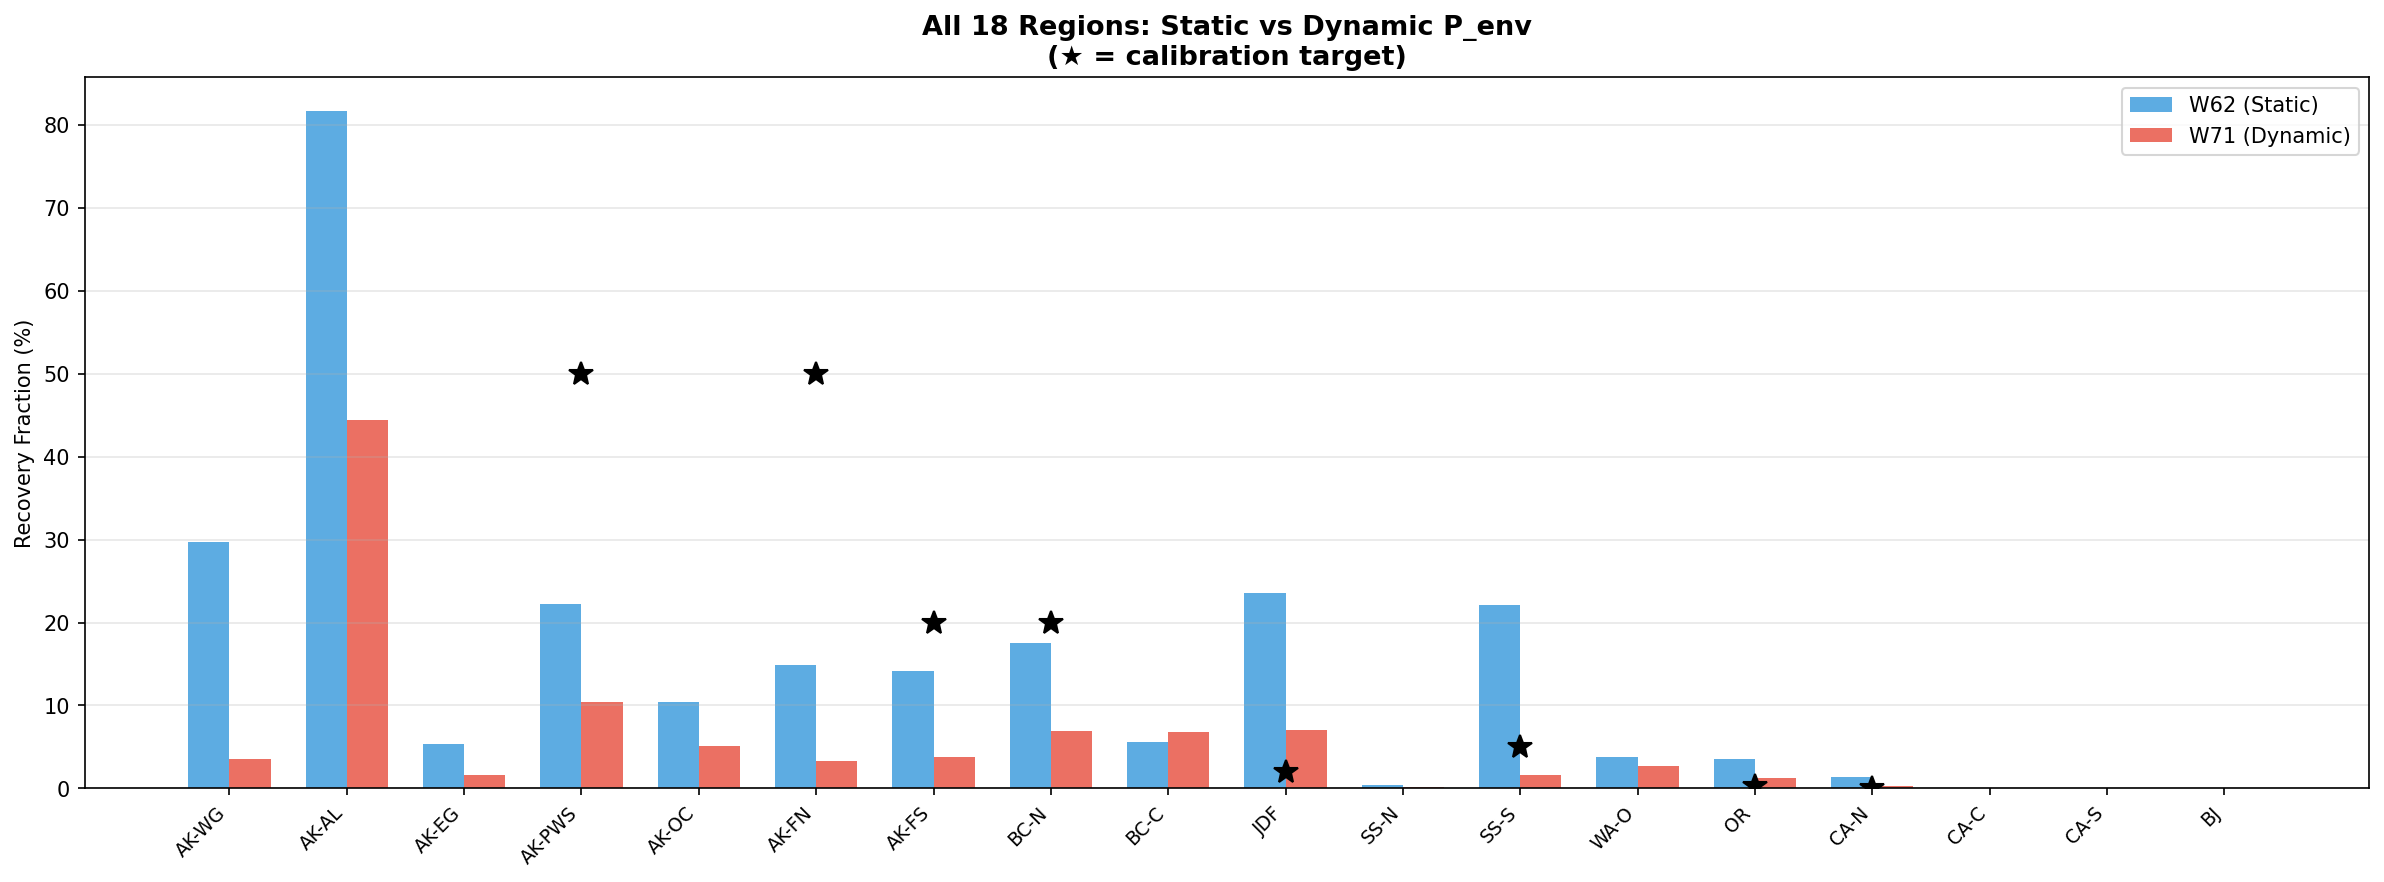
\includegraphics[width=\textwidth]{figures/fig8_all_regions.png}
\caption{All 18 regions: static (W62, blue) vs dynamic (W71, red). Stars mark calibration targets. Dynamic P\textsubscript{env} dramatically suppresses southern regions while partially preserving northern recovery. The gradient is clear across the full range.}
\end{figure}

\section{Demographic Dynamics (W71)}

\begin{figure}[H]
\centering
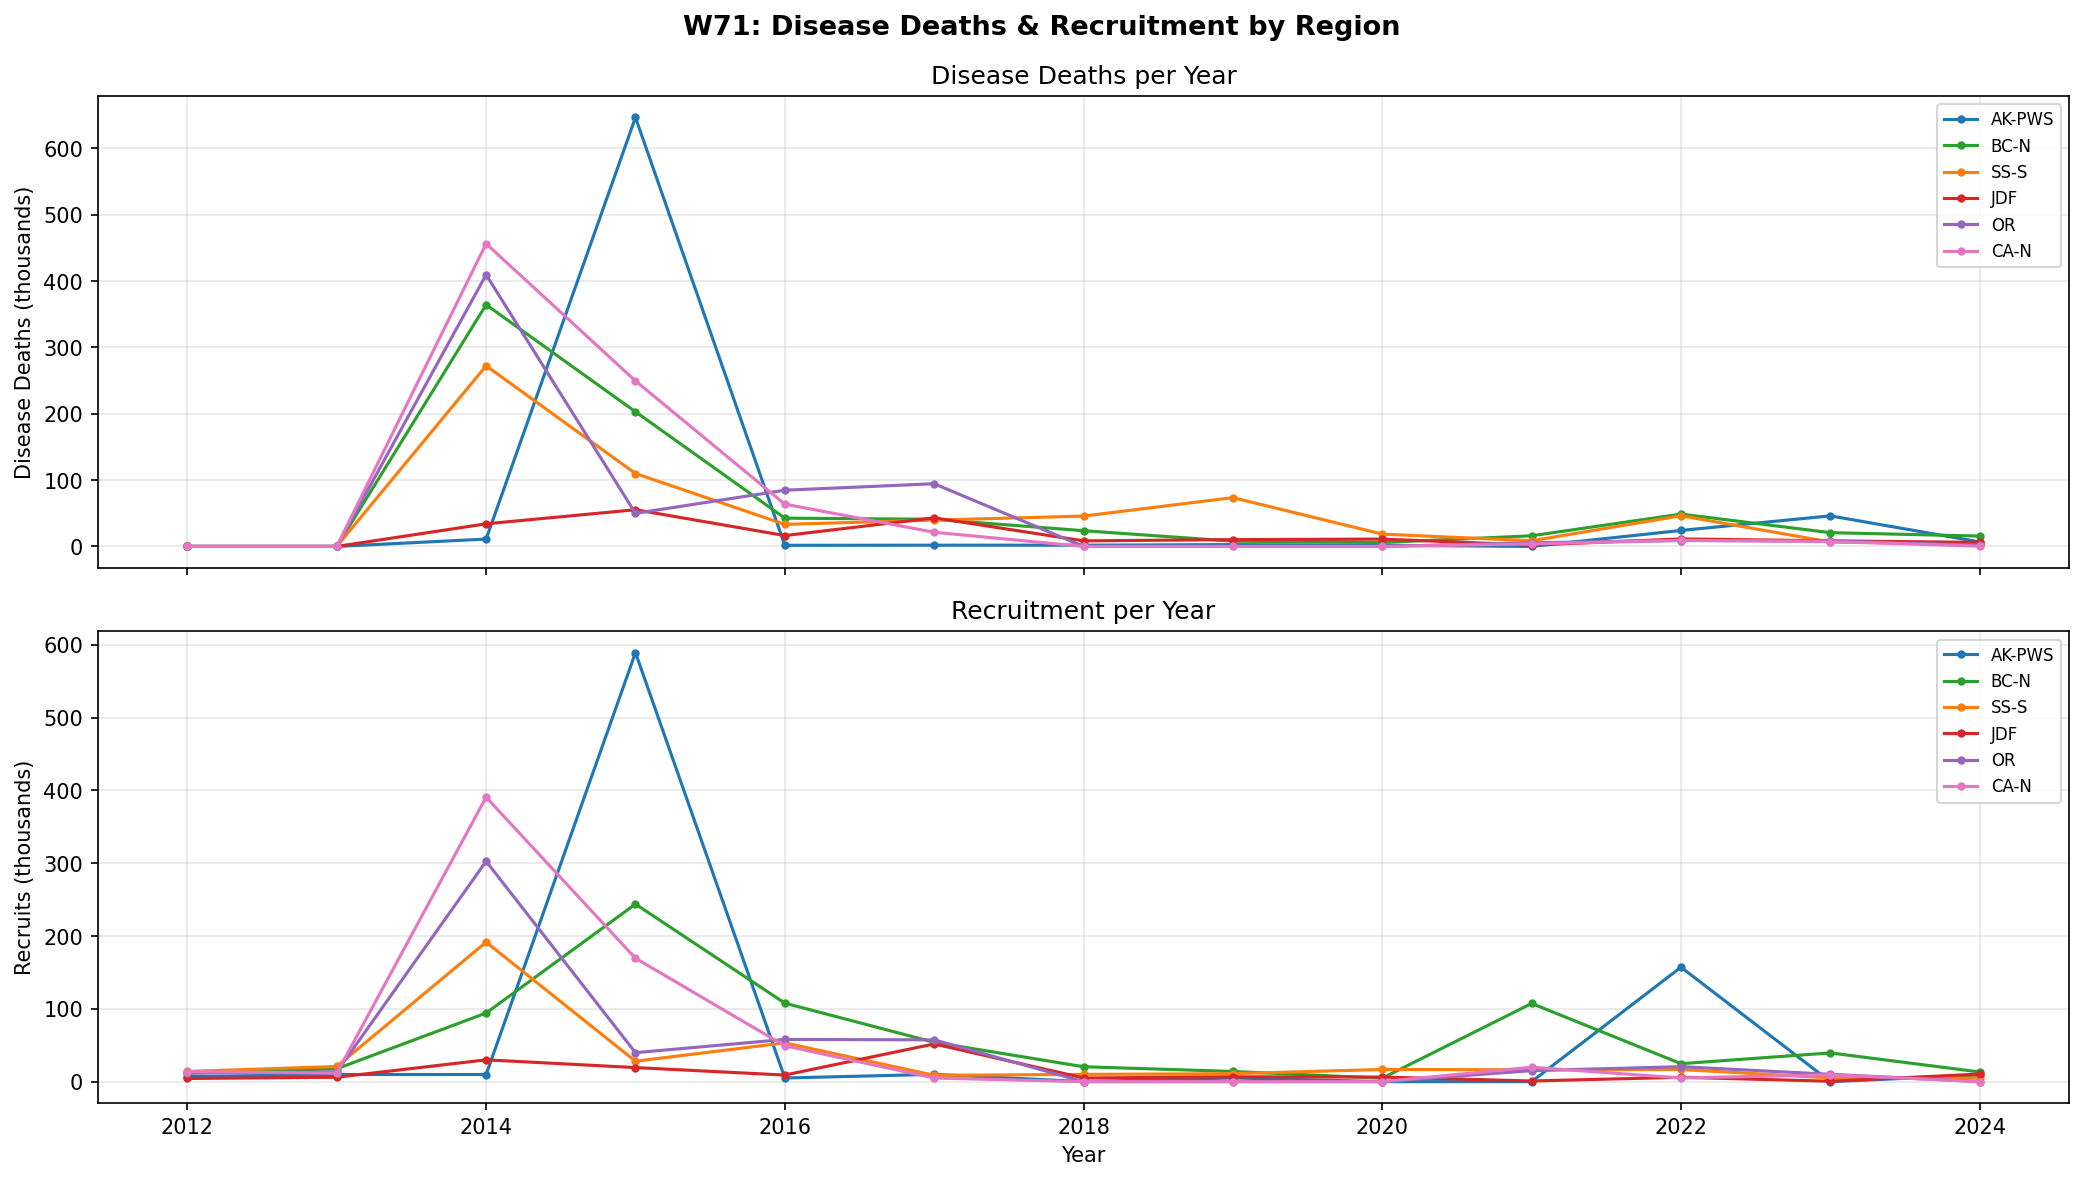
\includegraphics[width=\textwidth]{figures/fig7_deaths_recruits.png}
\caption{W71 disease deaths (top) and recruitment (bottom). AK-PWS (blue) shows massive death pulse at year 3--4, then minimal deaths. SS-S (orange) shows sustained disease deaths through year 10. Recruitment pulses correspond to recovery attempts --- note La Ni\~na-driven spikes in 2021.}
\end{figure}

\section{Genetic Evolution}

\begin{figure}[H]
\centering
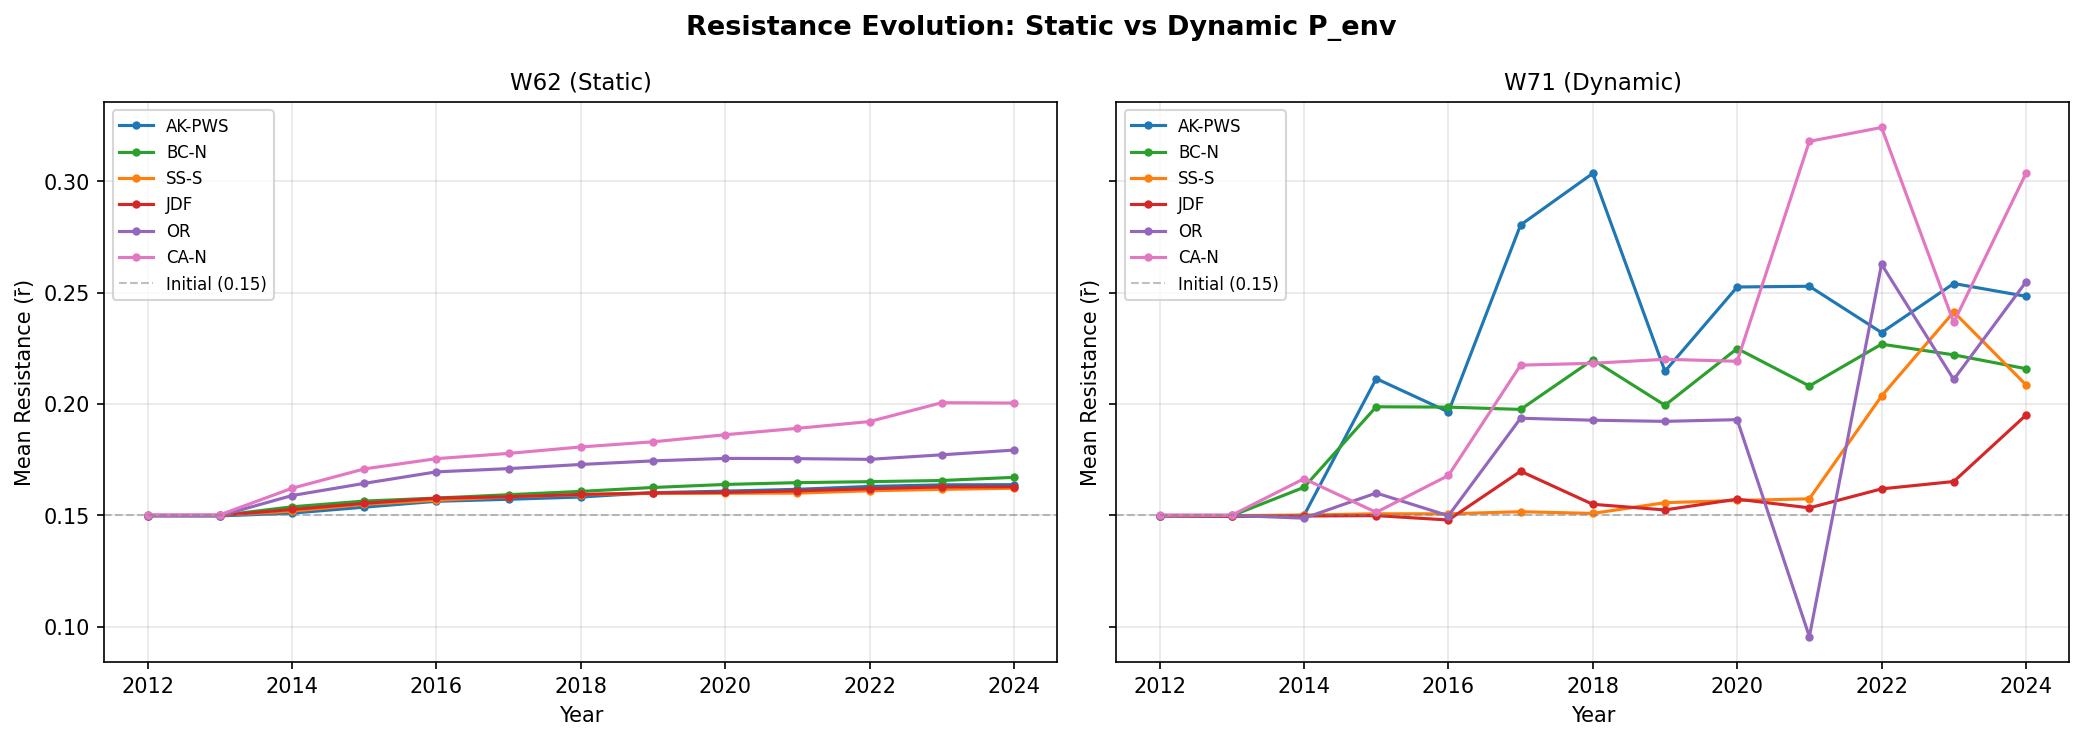
\includegraphics[width=\textwidth]{figures/fig5_resistance_evolution.png}
\caption{Resistance evolution comparison. Static P\textsubscript{env} (left): modest, uniform selection (all regions $r \approx 0.17$--0.22). Dynamic P\textsubscript{env} (right): AK-PWS shows rapid resistance increase ($r = 0.30$ by year 7), while SS-S evolves slowly --- population too suppressed for efficient selection.}
\end{figure}

\section{Year-by-Year Recovery Trajectories (W71)}

\begin{table}[H]
\centering
\small
\begin{tabular}{l|rrrrrrrrrrrrr}
\toprule
Region & Y1 & Y2 & Y3 & Y4 & Y5 & Y6 & Y7 & Y8 & Y9 & Y10 & Y11 & Y12 & Y13 \\
\midrule
AK-PWS & 100 & 100 & 95 & 1 & 1 & 3 & 2 & 2 & 1 & 1 & 36 & 12 & 10 \\
BC-N & 100 & 100 & 21 & 6 & 12 & 10 & 6 & 6 & 5 & 19 & 9 & 9 & 7 \\
SS-S & 100 & 100 & 71 & 48 & 48 & 39 & 29 & 13 & 11 & 11 & 3 & 2 & 2 \\
JDF & 100 & 100 & 88 & 54 & 46 & 39 & 33 & 28 & 21 & 20 & 13 & 7 & 7 \\
OR & 100 & 100 & 41 & 34 & 19 & 0 & 0 & 0 & 0 & 1 & 3 & 2 & 1 \\
CA-N & 100 & 99 & 54 & 14 & 6 & 0 & 0 & 0 & 0 & 4 & 1 & 0 & 0 \\
\bottomrule
\end{tabular}
\caption{Population as \% of pre-crash peak. South (CA-N, OR) crashes to 0\% and stays near-extinct. North (AK-PWS) crashes then shows La Ni\~na rebound at year 11. SS-S shows gradual decline from 71\% to 2\% --- sustained disease pressure from the SST-modulated floor.}
\end{table}

\section{Recommended Next Steps}

W71 demonstrates that dynamic P\textsubscript{env} solves the gradient problem. The remaining issue is overall recovery level --- everything is $\sim$3--5$\times$ too suppressed. Recommended:

\begin{enumerate}
    \item \textbf{Increase K$_{1/2}$}: W71 base (floor=100, $\delta$=0.02) with K$_{1/2}$ = [600K, 800K, 1M]. Higher K$_{1/2}$ gives populations more demographic resilience.
    \item \textbf{Lower P\textsubscript{env,max}}: Try 1000--1500 instead of 2000 to reduce initial crash severity.
    \item \textbf{Intermediate floor}: Try floor=75 with higher K$_{1/2}$.
    \item \textbf{Fine-tune $\alpha_\text{env}$ last}: It's a global intensity knob, not a gradient knob.
\end{enumerate}

\section{Conclusion}

Dynamic P\textsubscript{env} definitively solves the differential recovery problem. The SST-modulated community floor creates a 6.6$\times$ north-south gradient that was impossible with static P\textsubscript{env} (1.01$\times$ ratio). The mechanism is biologically grounded: environmental vibrio populations require host amplification to persist, and warm waters maintain higher baseline concentrations via the VBNC sigmoid. Next calibration round should adjust K$_{1/2}$ and P\textsubscript{env,max} to lift overall recovery while preserving the gradient.

\end{document}
